\documentclass[11pt]{article}

\usepackage{amsmath, amsthm, amssymb}
\usepackage{enumerate}
\usepackage{pdflscape}
\usepackage{caption}
\usepackage{bm}

\usepackage{ifpdf}
\ifpdf
\usepackage[pdftex]{graphicx}
\else
\usepackage[dvips]{graphicx}
\fi
\usepackage{tikz}
 	 \usetikzlibrary{arrows,backgrounds}
\usepackage[all]{xy}

\usepackage{multicol}

\usepackage{tocvsec2}

\usepackage{bbm}

\input xy
\xyoption{all}

\usepackage[pdftex,plainpages=false,hypertexnames=false,pdfpagelabels]{hyperref}
\newcommand{\arxiv}[1]{\href{http://arxiv.org/abs/#1}{\tt arXiv:\nolinkurl{#1}}}
\newcommand{\arXiv}[1]{\href{http://arxiv.org/abs/#1}{\tt arXiv:\nolinkurl{#1}}}
\newcommand{\doi}[1]{\href{http://dx.doi.org/#1}{{\tt DOI:#1}}}
\newcommand{\euclid}[1]{\href{http://projecteuclid.org/getRecord?id=#1}{{\tt #1}}}
\newcommand{\mathscinet}[1]{\href{http://www.ams.org/mathscinet-getitem?mr=#1}{\tt #1}}
\newcommand{\googlebooks}[1]{(preview at \href{http://books.google.com/books?id=#1}{google books})}
\newcommand{\Ws}{\text{W*}}

\usepackage{xcolor}
\definecolor{dark-red}{rgb}{0.7,0.25,0.25}
\definecolor{dark-blue}{rgb}{0.15,0.15,0.55}
\definecolor{medium-blue}{rgb}{0,0,.8}
\definecolor{shaded-blue}{RGB}{98,140,255}
\definecolor{DarkGreen}{RGB}{0,150,0}
\definecolor{rho}{named}{red}
\hypersetup{
   colorlinks, linkcolor={purple},
   citecolor={medium-blue}, urlcolor={medium-blue}
}

%\addtolength{\textwidth}{.5in}
\usepackage{longtable}
\usepackage{fullpage}
%\renewcommand{\arraystretch}{1.5}

% Page size %%%%%%%%%%%%%%%%%%%%%%%%%%%%%%%%%%%%%%%%%%%
\setlength\topmargin{-.25in}
\setlength\headheight{0in}
\setlength\headsep{.2in}
\setlength\textheight{9in}
%\addtolength{\hoffset}{-0.25in}
%\addtolength{\textwidth}{.5in}
\setlength\parindent{0.25in}

% Theorems %%%%%%%%%%%%%%%%%%%%%%%%%%%%%%%%%%%%%%%%%%
\theoremstyle{plain}
\newtheorem{thm}{Theorem}[section]
\newtheorem*{thm*}{Theorem}
\newtheorem{thmalpha}{Theorem}
\renewcommand*{\thethmalpha}{\Alph{thmalpha}}
\newtheorem{cor}[thm]{Corollary}
\newtheorem{coralpha}[thmalpha]{Corollary}
\newtheorem*{cor*}{Corollary}
\newtheorem{conj}[thm]{Conjecture}
\newtheorem{conjalpha}[thmalpha]{Conjecture}
\newtheorem*{conj*}{Conjecture}
\newtheorem{lem}[thm]{Lemma}
\newtheorem{fact}[thm]{Fact}
\newtheorem{facts}[thm]{Facts}
\newtheorem{prop}[thm]{Proposition}
\newtheorem{quest}[thm]{Question}
\newtheorem*{quest*}{Question}
\newtheorem*{claim*}{Claim}
\newtheorem{quests}[thm]{Questions}
\theoremstyle{definition}
\newtheorem{defn}[thm]{Definition}
\newtheorem{construction}[thm]{Construction}
\newtheorem{alg}[thm]{Algorithm}
\newtheorem{assumption}[thm]{Assumption}
\newtheorem{nota}[thm]{Notation}
\newtheorem{nb}[thm]{Note}
\newtheorem{note}[thm]{Note}
\newtheorem{exs}[thm]{Examples}
\newtheorem{ex}[thm]{Example}
\newtheorem{exercise}[thm]{Exercise}
\newtheorem{sub-ex}[thm]{Sub-Example}
\newtheorem{rem}[thm]{Remark}
\newtheorem*{rem*}{Remark}
\newtheorem{remark}[thm]{Remark}
\newtheorem{rems}[thm]{Remarks}
\newtheorem{warn}[thm]{Warning}

% Figure Numbering %%%%%%%%%%%%%%%%%%%%%%%%%%%%%%%%%%%
\usepackage{chngcntr} %Numbers figures by section
\counterwithin{figure}{section}

% Operators %%%%%%%%%%%%%%%%%%%%%%%%%%%%%%%%%%%%%%%%%%%
\DeclareMathOperator{\Ad}{Ad}
\DeclareMathOperator{\Aut}{Aut}
\DeclareMathOperator{\coev}{coev}
\DeclareMathOperator{\Dom}{Dom}
\DeclareMathOperator{\End}{End}
\DeclareMathOperator{\ev}{ev}
\DeclareMathOperator{\Hom}{Hom}
\DeclareMathOperator{\Mor}{Mor}
\DeclareMathOperator{\op}{op}
\DeclareMathOperator{\ONB}{ONB}
\DeclareMathOperator{\Ob}{Ob}
\DeclareMathOperator{\rev}{rev}
\DeclareMathOperator{\spann}{span}
\DeclareMathOperator{\supp}{supp}
\DeclareMathOperator{\id}{id}
\DeclareMathOperator{\Isom}{Isom}
\DeclareMathOperator{\ind}{ind}
\DeclareMathOperator{\im}{im}
\DeclareMathOperator{\Irr}{Irr}
\DeclareMathOperator{\Spec}{Spec}
\DeclareMathOperator{\Stab}{Stab}
\DeclareMathOperator{\Tr}{Tr}
\DeclareMathOperator{\tr}{tr}
\DeclareMathOperator{\Gr}{Gr}


% Math %%%%%%%%%%%%%%%%%%%%%%%%%%%%%%%%%%%%%%%%%%%%%
\newcommand{\D}{\displaystyle}
\newcommand{\comment}[1]{}
\newcommand{\hs}{\hspace{.07in}}
\newcommand{\hsp}[1]{\hs\text{#1}\hs}
\newcommand{\be}{\begin{enumerate}[label=(\arabic*)]}
\newcommand{\ee}{\end{enumerate}}
\newcommand{\itm}[1]{\item[\underline{\ensuremath{#1}:}]}
\newcommand{\itt}[1]{\item[\underline{\text{#1}:}]}
\newcommand{\N}{\mathbb{N}}
\newcommand{\Natural}{\mathbb{N}}
\newcommand{\Z}{\mathbb{Z}}
\newcommand{\Q}{\mathbb{Q}}
\newcommand{\F}{\mathbb{F}}
\newcommand{\R}{\mathbb{R}}
\newcommand{\C}{\mathbb{C}}
\newcommand{\B}{\mathbb{B}}
\renewcommand{\P}{\mathbb{P}}
\newcommand{\I}{\infty}
\newcommand{\set}[2]{\left\{#1 \middle| #2\right\}}
\newcommand{\thh}{^{\text{th}}}
\renewcommand{\a}{\mathfrak{a}}
\renewcommand{\b}{\mathfrak{b}}
\renewcommand{\c}{\mathfrak{c}}
\newcommand{\n}{\mathfrak{n}}
\newcommand{\m}{\mathfrak{m}}
\newcommand{\bbOne}{\mathbbm{1}}
\renewcommand{\alg}[1]{{\bm{\langle} #1\bm{\rangle}}}


% some math commands specific to this document %%%%%%%%%%%%
\newcommand{\xalt}{x^{\text{alt}\otimes n}}
\newcommand{\xbaralt}{\overline{x}^{\text{alt}\otimes n}}
\newcommand{\act}{\overline{x}^{?}}
%%%%%%%%%%%%%%%%%%%%%%%%%%%%

\newcommand{\dave}[1]{\marginpar{\tiny \textcolor{orange}{DP: #1}}}
\newcommand{\corey}[1]{\marginpar{\tiny \textcolor{green}{CJ: #1}}}
\newcommand{\Af}{\mathcal{A}\Lambda_{F}}
\newcommand{\WStar}{\bfW\text{*}}
%\newcommand{\Irr}{\text{Irr}(\mathcal{C})}

% tricky way to iterate macros over a list
\def\semicolon{;}
\def\applytolist#1{
    \expandafter\def\csname multi#1\endcsname##1{
        \def\multiack{##1}\ifx\multiack\semicolon
            \def\next{\relax}
        \else
            \csname #1\endcsname{##1}
            \def\next{\csname multi#1\endcsname}
        \fi
        \next}
    \csname multi#1\endcsname}

% \def\cA{{\cal A}} for A..Z
\def\calc#1{\expandafter\def\csname c#1\endcsname{{\mathcal #1}}}
\applytolist{calc}QWERTYUIOPLKJHGFDSAZXCVBNM;
% \def\bbA{{\mathbb A}} for A..Z
\def\bbc#1{\expandafter\def\csname bb#1\endcsname{{\mathbb #1}}}
\applytolist{bbc}QWERTYUIOPLKJHGFDSAZXCVBNM;
% \def\bfA{{\mathbf A}} for A..Z
\def\bfc#1{\expandafter\def\csname bf#1\endcsname{{\mathbf #1}}}
\applytolist{bfc}QWERTYUIOPLKJHGFDSAZXCVBNM;
% \def\sA{{\sf A}} for A..Z
\def\sfc#1{\expandafter\def\csname s#1\endcsname{{\sf #1}}}
\applytolist{sfc}QWERTYUIOPLKJHGFDSAZXCVBNM;
% \def\fA{{\mathfrak A}} for A..Z
\def\fc#1{\expandafter\def\csname f#1\endcsname{{\mathfrak #1}}}
\applytolist{fc}QWERTYUIOPLKJHGFDSAZXCVBNM;


\newcommand{\PA}{\cP\hspace{-.1cm}\cA}
\newcommand{\Fun}{{\sf Fun}}
\newcommand{\Rep}{{\sf Rep}}
\newcommand{\Set}{{\sf Set}}
\newcommand{\FreeMod}{{\sf FreeMod}}
\newcommand{\Mod}{{\sf Mod}}
\newcommand{\Proj}{{\sf Proj}}
\newcommand{\AlgBim}{{\sf AlgBim}}
\newcommand{\Bim}{{\sf Bim}}
\newcommand{\bfBim}{{\sf Bim_{bf}}}
\newcommand{\spBim}{{\sf Bim^{sp}}}
\newcommand{\spbfBim}{{\sf Bim_{bf}^{sp}}}
\renewcommand{\Vec}{{\sf Vec}}
\newcommand{\fdVec}{{\sf Vec_{fd}}}
\newcommand{\Hilb}{{\sf Hilb}}
\newcommand{\fdHilb}{{\sf Hilb_{fd}}}
\newcommand{\ConAlg}{{\sf ConAlg}}
\newcommand{\DisInc}{{\sf DisInc}}


\newcommand{\jw}[1]{f^{(#1)}}
\newcommand{\todo}[1]{\textcolor{blue}{\textbf{TODO: #1}}}
\newcommand{\nn}[1]{\textcolor{red}{[[#1]]}}
\newcommand{\noshow}[1]{}
\newcommand{\MR}[1]{}
\newcommand{\TL}{\cT\hspace{-.08cm}\cL}
\newcommand{\rhoE}{\textcolor{rho}{e_1}}
\newcommand{\rhoJW}{\textcolor{rho}{\jw{2}}}


% TikZ operators %%%%%%%%%%%%%%%%%%%%%%%%%%%%%%%%%%%%%%%%
\usetikzlibrary{shapes}
\usetikzlibrary{cd}
\usetikzlibrary{backgrounds}
\usetikzlibrary{decorations,decorations.pathreplacing,decorations.markings}
\usetikzlibrary{fit,calc,through}
\usetikzlibrary{external}
\usetikzlibrary{arrows}
\tikzset{vertex/.style = {shape=circle,draw,fill=black,inner sep=0pt,minimum size=5pt}}
\tikzset{edge/.style = {->,> = latex', bend right}}
\tikzset{
	super thick/.style={line width=3pt}
}
\tikzset{
    quadruple/.style args={[#1] in [#2] in [#3] in [#4]}{
        #1,preaction={preaction={preaction={draw,#4},draw,#3}, draw,#2}
    }
}
\tikzstyle{shaded}=[fill=shaded-blue]
\tikzstyle{unshaded}=[fill=white]
\tikzstyle{empty box}=[circle, draw, thick, fill=white, opaque, inner sep=2mm]
\tikzstyle{annular}=[scale=.7, inner sep=1mm, baseline]
\tikzstyle{rectangular}=[scale=.75, inner sep=1mm, baseline=-.1cm]
\tikzstyle{mid>}=[decoration={markings, mark=at position 0.5 with {\arrow{>}}}, postaction={decorate}]
\tikzstyle{mid<}=[decoration={markings, mark=at position 0.5 with {\arrow{<}}}, postaction={decorate}]
\tikzstyle{over}=[double, draw=white, super thick, double=]

\newcommand{\roundNbox}[6]{
	\draw[rounded corners=5pt, very thick, #1] ($#2+(-#3,-#3)+(-#4,0)$) rectangle ($#2+(#3,#3)+(#5,0)$);
	\coordinate (ZZa) at ($#2+(-#4,0)$);
	\coordinate (ZZb) at ($#2+(#5,0)$);
	\node at ($1/2*(ZZa)+1/2*(ZZb)$) {#6};
}


\newcommand{\nbox}[6]{
	\draw[thick, #1] ($#2+(-#3,-#3)+(-#4,0)$) rectangle ($#2+(#3,#3)+(#5,0)$);
	\coordinate (ZZa) at ($#2+(-#4,0)$);
	\coordinate (ZZb) at ($#2+(#5,0)$);
	\node at ($1/2*(ZZa)+1/2*(ZZb)$) {#6};
}

\newcommand{\ncircle}[4]{
	\draw[very thick, #1] #2 circle (#3);
	\node at #2 {#4};
%	\filldraw[red] ($#2+(#4:#3cm)$) circle (.05cm);
%	\node at ($#2+(#4:.15cm)+(#4:#3cm)$) {$\star$};
}

  \newcommand{\tikzmath}[2][]
     {\vcenter{\hbox{\begin{tikzpicture}[#1]#2
                     \end{tikzpicture}}}
     }

% colors %%%%%%%%%%%%%%%%%%%%%%%%%%%%%%%%%%%%%%%%
\newcommand{\cupcolor}{DarkGreen}
\newcommand{\alphacolor}{blue}
\newcommand{\betacolor}{red}

% title %%%%%%%%%%%%%%%%%%%%%%%%%%%%%%%%%%%%%%%%%

\title{The Embedding Theorem for Module Categories}
\author{Desmond Coles, Peter Huston, David Penneys, \& Srivatsa Srinivas}





%%%%%%%%%%%%%%%%%%%%%%%%%%%%%%%%%%%%%%


\usepackage[utf8]{inputenc}
\begin{document}


%%%%%%%%%%%%%%%%%%%%%%%%%%%%%%%%%%%%%%%%%%%%%%%%%%%%%%%%%%%%%%%
%%%%%%%%%%%%%%%%%%%%%%%%%%%%%%%%%%%%%%%%%%%%%%%%%%%%%%%%%%%%%%%
%%%%%%%%%%%%%%%%%%%%%%%%%%%%%%%%%%%%%%%%%%%%%%%%%%

\maketitle
\begin{abstract}
Please read our paper it's great, like really really great seriously please.
\end{abstract}
\section{Introduction}
\section{Preliminaries}
\subsection{Planar Algebras and the Paragroup}
Planar algebras were originally introduced in \cite{planaralg1}, we will use the same definitions and conventions as \cite{penneys}, \cite{peters}, \cite{jones}, and \cite{planaralg2}. The reader is referred to these references for further information on planar algebras. From any subfactor planar algebra one may construct a 2-category from it, we refer the reader to \cite{paragroup} and \cite{paragroup2} for more details, we will refer to the definitions used in \cite{paragroup} as we wish to work with shaded planar algebras.

\begin{defn}\textnormal{
Let $Q_{\bullet}$ be a subfactor planar algebra, we will define a 2-category $\cG$ called the \textit{paragroup}.
\begin{itemize}
\item The 0-morphisms of $\cG$ are the two objects
$
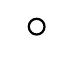
\begin{tikzpicture}
\draw[thick] (0,0) circle (1mm) ;
\end{tikzpicture}
$ 
and
$

\begin{tikzpicture}
\filldraw[thick][shaded] (0,0) circle (1mm);
\end{tikzpicture}
$.
\item The 1-morphisms are projections in the box spaces of $Q_{\bullet}$ and are given as follows:
\begin{itemize}
\item $\Hom_{\cG}(
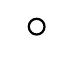
\begin{tikzpicture}
\draw[thick] (0,0) circle (1mm) ;
\end{tikzpicture}
\rightarrow
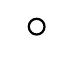
\begin{tikzpicture}
\draw[thick] (0,0) circle (1mm) ;
\end{tikzpicture})=
\{p\in Q_{i,+}|\text{$p$ is projection and $i$ is even}\}
$
\item $\Hom_{\cG}(
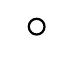
\begin{tikzpicture}
\draw[thick] (0,0) circle (1mm) ;
\end{tikzpicture}
\rightarrow

\begin{tikzpicture}
\filldraw[thick][shaded] (0,0) circle (1mm);
\end{tikzpicture})
=
\{p\in Q_{i,+}|\text{$p$ is projection and $i$ is odd}\}
$
\item $\Hom_{\cG}(

\begin{tikzpicture}
\filldraw[thick][shaded] (0,0) circle (1mm);
\end{tikzpicture}
\rightarrow
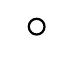
\begin{tikzpicture}
\draw[thick] (0,0) circle (1mm) ;
\end{tikzpicture})
=
\{p\in Q_{i,-}|\text{$p$ is projection and $i$ is odd}\}
$
\item $\Hom_{\cG}(

\begin{tikzpicture}
\filldraw[thick][shaded] (0,0) circle (1mm);
\end{tikzpicture}
\rightarrow

\begin{tikzpicture}
\filldraw[thick][shaded] (0,0) circle (1mm);
\end{tikzpicture})=
\{p\in Q_{i,-}|\text{$p$ is projection and $i$ is even}\}
$
\end{itemize}
Composition is denoted by $\otimes$ and is represented diagrammatically by horizontal concatenation of diagrams.
\item The 2-morphisms of $\cG$ are defined as follows, for $p\in P_{i,\pm}$ and $q\in P_{i,\pm}$ then $\Hom_{\cG}(p\rightarrow q)=qP_{j\rightarrow i}p$ and $P_{j\rightarrow i}$ is $P_{i+j}$ with elements represented $j$ with strings emanating from the top and $i$ from the bottom. If $i$ and $j$ don't have the same parity this does not exist to we take the morphisms to be zero.
\end{itemize}}
\end{defn}

For a general subfactor planar algebra $Q_{\bullet}$ $\cG$ can be interpreted as a semisimple multitensor category in the sense of \cite{egno}. When $Q_{\bullet}$ is of finite depth $\cG$ is in fact a $2\times 2$ multitensor category.
\subsection{Markov Sequences}


\begin{defn}
A \emph{Markov sequence} consists of a sequence $(M_n, \tr_n)_{n\geq 0}$ of finite dimensional von Neumann algebras, such that $M_n$ is unitally included in $M_{n_1}$, each $M_n$ has a faithful normal tracial states such that $\tr_{n+1}|_{M_n} = \tr_n$ for all $n\geq 0$, and a sequence of \emph{Jones projections} $e_n \in M_{n+1}$ for all $n\geq 1$ such that:
\begin{itemize}
\item
The projections $(e_n)$ satisfy the Temperley-Lieb-Jones relations:
\begin{enumerate}[(1)]
\item
$e_i^2 = e_i = e_i^*$ for all $i$,
\item
$e_i e_j = e_j e_i$ for $|i-j|>1$, and
\item
there is a fixed constant $d>0$ such that $e_{i} e_{i\pm 1} e_i = d^{-2} e_i$ for all $i$.
\end{enumerate}
\item
For all $x\in M_n$, $e_n x e_n = E_n(x)e_n$ where $E_n: M_n \to M_{n-1}$ is the canonical faithful trace-preserving conditional expectation.
\item
For all $n\geq 1$, $E_{n+1}(e_n) = d^{-2}$.
\item
(pull down)
For all $n\geq 1$, $M_{n+1}e_n = M_n e_n$.

\end{itemize}
\end{defn}


\begin{rem}
$M_n e_n M_n$ is a 2-sided ideal in $M_{n+1}$ for all $n\geq 1$ iff the pull down condition holds. Indeed if the pull down condition holds then $M_{n+1} M_n e_n M_n \subseteq M_{n+1} e_n M_n = M_n e_n M_n$, and the same argument holds on the right by first taking adjoints. Conversely, if $M_n e_n M_n$ is a 2-sided ideal, then $M_{n+1} e_n = (M_{n+1} e_n)e_n \subseteq (M_n e_n M_n) e_n = M_n e_n$.
\end{rem}




\begin{prop} Markov sequence satisfies the following elementary properties for $n\geq 1$.
\begin{enumerate}[(A)]
\item
\label{EP:injective}
The map $M_{n}\ni y\mapsto ye_n \in M_{n+1}$ is injective.

\item
\label{EP:UniquePullDown}
For all $x\in M_{n+1}$, $d^{2}E_{n+1}(x e_n)$ is the unique element $y\in M_n$ such that $x e_n = ye_n$ \cite[Lem.~1.2]{MR860811}.

\item
\label{EP:MarkovTraces}
The traces $\tr_{n+1}$ satisfy the following \emph{Markov property} with respect to $M_n$ and $e_n$: for all $x\in M_n$, $\tr_{n+1}(xe_n) = d^{-2} \tr_n(x)$.

\item
\label{EP:CompressM_{n+1}}
$e_n M_{n+1}e_n = M_{n-1}e_n$.

\item
\label{EP:2SidedIdeal}
$X_{n+1}:=M_n e_n M_n$ is a 2-sided ideal of $M_{n+1}$, and thus $M_{n+1}$ splits as a direct sum of von Neumann algebras $X_{n+1}\oplus Y_{n+1}$.
(In \cite[Thm.~4.1.4 and Thm.~4.6.3]{MR999799}, $Y_{n+1}$ is the so-called `new stuff'.)
By convention, we define $Y_0 = M_0$ and $Y_1 = M_0$, so that $X_0 = (0)$ and $X_1 = (0)$.

\item
\label{EP:BasicContruction}
The map $ae_n b\mapsto ap_n b$ gives a $*$-isomorphism from $X_{n+1}=M_n e_n M_n$ to $\langle M_n , p_n\rangle=M_np_nM_n$, the Jones basic construction of $M_{n-1} \subseteq M_n$ acting on $L^2(M_n,\tr_n)$.

\item
\label{EP:OtherMarkovDef}
Under the isomorphism $X_{n+1} \cong M_n p_n M_n$, the canonical non-normalized trace $\Tr_{n+1}$ on the Jones basic construction algebra $M_np_nM_n$ satisfying $\Tr_{n+1}(ap_nb) = \tr_n(ab)$ for $a,b\in M_n$ equals $d^2 \tr_{n+1}|_{X_{n+1}}$.

\item
\label{EP:NewStuff}
If $y\in Y_{n+1}$ and $x\in X_{n}$, then $yx = 0$ in $M_{n+1}$.
Hence $E_{n+1}(Y_{n+1}) \subseteq Y_{n}$.
(``The new stuff comes only from the old new stuff" \cite{MR999799}.)

\item
\label{EP:FiniteDepth}
If $Y_n =(0)$, then $Y_{k} = (0)$ for all $k\geq n$.

\end{enumerate}
\end{prop}

\begin{proof} 

\begin{enumerate}[(A)]
\item

We know that $d^2E_{n+1}(ye_n) = y $ so the proposed map has a left inverse.

\item

If $xe_n = ye_n$ for $y\in M_n$,  $E_{n+1}(xe_n) = E_{n+1}(y e_n) = y E_{n+1}(e_n) = d^{-2} y$, and the map $M_n\ni z\mapsto ze_n\in M_{n+1}$ is injective.

\item

For $x\in M_n$, $\tr_{n+1}(xe_n) = \tr_n(E_{n+1}(xe_n)) = \tr_n(x E_{n+1}(e_n)) = d^{-2} \tr_n(x)$ since $E_{n+1}(e_n) = d^{-2}$.

\item

$M_{n+1} e_n = M_n e_n$ and $e_nxe_n = E_n(x)e_n$ for all $x\in M_n$.

\item

$M_ne_nM_n$ is a 2-sided ideal of $M_{n+1}$ by the pull down condition.

\item

It suffices to show the map is injective, which shows it is well-defined.
Suppose $\sum a_i p_n b_i = 0$.
Then for all $a,b\in M_n$, we have $0=p_na\left(\sum a_i p_n b_i\right) bp_n = \sum E_{n}(aa_i)E_n(b_ib)p_n$, which implies $\sum E_{n}(aa_i)E_n(b_ib) = 0$ as $M_n \ni x\mapsto xp_n \in \langle M_n, p_n\rangle$ is injective.
Hence $0 = \sum E_{n}(aa_i)E_n(b_ib)e_n = e_na\left(\sum a_i e_n b_i\right) be_n$ for all $a,b\in M_n$, which implies $\sum a_i e_n b_i = 0$.

\item

For $a,b\in M_n$, 
$\Tr_{n+1}(ap_n b) = \tr_n(ab) = \tr_n(ba) = d^2\tr_{n+1}(bae_n) = d^2 \tr_{n+1}(ae_n b)$.

\item

Since $X_0 = (0)$ and $X_1 = (0)$ by definition, we may assume $n\geq 2$.
As in the proof of \cite[Thm.~4.6.3.vi]{MR999799} and (5), we may assume $y$ is a central projection in $M_{n+1}$ such that $y e_{n} = 0$.
Then for all $ae_{n-1} b \in X_n$, $y ae_n b = d^2 yae_n e_{n+1}e_n b = d^2 ae_n ye_{n+1} e_n b = 0$.
The final claim follows from $z_{n}E_{n+1}(y) = E_{n+1}(z_n y)= 0$ where $z_n$ is the central support of $e_{n-1}$ in $M_n$.

\item

This follows immediately from the previous fact.

\end{enumerate}

\end{proof}


Notice that by \ref{EP:BasicContruction} the Bratteli diagram for the inclusion $M_{n}\subset M_{n+1}$ consists of the reflection of the Bratteli diagram for the inclusion $M_{n-1} \subset M_n$, together with possibly some new edges and vertices corresponding to simple summands of $Y_{n+1}$. By \ref{EP:NewStuff}, the new vertices at level $n+1$ only connect to the vertices that were new at level $n$. This leads to the following definition:


\begin{defn}
The \emph{principal graph} of the Markov sequence $(M_n,\tr_n)$ with Jones projections $(e_n)$ consists of the \emph{new} vertices at every level $n$ of the Bratteli diagram, together with all the edges connecting them.

The sequence is said to have \emph{finite depth} if the principal graph is finite.
\end{defn}


It follows then that the Markov sequence has finite depth if and only if there is an $n\in \bbN$ such that $Y_n = (0)$ as in Elementary Property \eqref{EP:FiniteDepth}. If a Markov sequence has finite depth then let $n\in \bbN$ be such that $Y_n=(0)$. Note that the Bratteli diagram for $M_0\subseteq M_1$ is part of the principal graph and the Bratteli diagram for $M_1\subseteq M_2$ is the Bratteli diagram for $M_0\subseteq M_1$ reflected upwards along with some new edges between the vertices corresponding to $Y_1$ and $Y_2$. So there is a natural isomorphism between the Bratteli diagram for $M_1\subseteq M_2$ and the subgraph of principal graph given only by the inclusions $M_0\subseteq M_1\subseteq M_2$. Similarly we can naturally identify the Bratteli diagram of $M_2\subseteq M_3$ with the subgraph of principal graph given only by the inclusions $M_0\subseteq M_1\subseteq M_2\subseteq M_3$. Continuing on this way we see that we have a natural identification of the prinicapl graph with the Bratteli diagram of $M_n\subseteq M_{n+1}$, and for $k\geq n$ the Bratteli diagram of $M_{k}\subset M_{k+1}$ is the bratelli diagram of $M_{k-1}\subset M_{k}$ (possibly reflected). This gives the following proposition:

\begin{prop}\label{BratteliPrincipal}
If a Markov sequence has finite depth then let $n\in \bbN$ be such that $Y_n=(0)$. Then if $k\geq n$ there is a canonical graph isomorphism between the principal graph of the sequence and the Bratteli diagram for $M_{k}\subset M_{k+1}$.
\end{prop}

\begin{ex}
The Temperley-Lieb algebras of modulus $d\geq 2$ with the usual Jones projections form a Markov sequence. The principal graph is $A_{\infty}$.
\end{ex}

\section{Construction of the Planar Algebra Associated to a Module Category}
\subsection{Construction of a Markov Sequence}
Given a subfactor planar algebra $Q_{\bullet}$, let $\cC$ be the paragroup of $Q_{\bullet}$ and $\cM$ be an indecomposable module category for $\cC$. We know that there is a $3\times 3$ unitary multifusion category $\widetilde{\cC}$, with $1_{\widetilde{\cC}}= 1_0 \oplus 1_1 \oplus 1_2$ and $\cC$ the  non-unital $2\times 2$ unitary multifusion subcategory with $1_\cC = 1_0\oplus 1_1$, so that $\cM\cong\cC_{20}\oplus \cC_{21}$. Overall,
$$
\cM 
=
\begin{pmatrix}
\cC_{20} & \cC_{21} 
\end{pmatrix}
\qquad\qquad
\cC
=
\begin{pmatrix}
\cC_{00} & \cC_{01} 
\\
\cC_{10} & \cC_{11}
\end{pmatrix}
\subset
\begin{pmatrix}
\cC_{00} & \cC_{01} & \cC_{02}
\\
\cC_{10} & \cC_{11} & \cC_{12}
\\
\cC_{20} & \cC_{21} & \cC_{22}
\end{pmatrix}
=
\widetilde{\cC}
$$
Let $x\in \cC_{01}$ be the strand pictured below:
$$x=

\begin{tikzpicture}[baseline=-.1cm]
	\fill[white] (0,-.7) rectangle (-.7,-.7);
	\fill[gray!25!white] (0,-.7) rectangle (.7,.7);
	\draw (0,-.7) -- (0,.7);

\end{tikzpicture}
\ \,\,\,\,\, \text{and,}\,\,\,\,\, \overline{x}=

\begin{tikzpicture}[baseline=-.1cm]
	\fill[white] (0,-.7) rectangle (.7,.7);
	\fill[gray!25!white] (0,-.7) rectangle (-.7,.7);
	\draw[fill] (0,-.7) -- (0,.7);

\end{tikzpicture}
\,\,\,\,\, \text{so} \,\,\,\,\, x\otimes \overline{x} = 
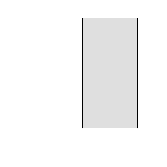
\begin{tikzpicture}[baseline=-.1cm]
	\fill[white] (0,-.7) rectangle (-.7,.7);
	\fill[gray!25!white] (0,-.7) rectangle (.7,.7);
	\draw (0,-.7) -- (0,.7);
	\draw (.7,-.7) -- (.7,.7);

\end{tikzpicture}
$$
By construction, $x$ is a generating object for $\cC$. If we pick a simple object $m\in \cC_{20}$, since $\cM$ is indecomposable, we have that any object of $\cM$ is isomorphic to a direct summand of $m\otimes \xalt$ for some nonnegative integer $n$, where $$
x^{\text{alt}\otimes n}:=\underbrace{x\otimes \overline{x} \otimes x \otimes \cdots \otimes x^?}_{n \text{ tensorands}}\,,
$$ and $x^? = \overline x$ if $n$ is even and $x$ if $n$ is odd. We define $\xbaralt$ similarly.

We will construct a finite depth Markov sequence of algebras from the action of $\cC$ on $\cM$ as follows. Set $A_n=\End_{\cC}(m\otimes \xalt)$. We can represent morphisms in $A_n$ as 
$$
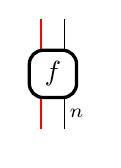
\begin{tikzpicture}[baseline=.4cm]
	\draw[thick, red] (-.15,-.7) -- (-.15,.7);
	\draw (.15,-.7) -- (.15,.7);
	
	\roundNbox{unshaded}{(0,0)}{.3}{0}{0}{$f$}
	
	\node at (.3,-.5) {\scriptsize{$n$}};

\end{tikzpicture}
$$
where the red strand represents $m$ and the $n$ represents $x^{\text{alt}\otimes n}$. We have a faithful tracial state $\tr_n:A_n\to \C$ given by
\begin{equation}\label{eq:TraceAn}
\tr_n(f) 
\,:=\, 
\frac{1}{\dim_\cC(m)\dim_\cC(x)^n}\cdot\tr_\cC(f)
\,=\,
\frac{1}{\dim_\cC(m)}\cdot
\frac{1}{d^n}
\cdot
\left(
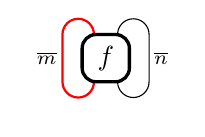
\begin{tikzpicture}[baseline=-.1cm, rotate=90]
	\draw[thick, red] (-.3,.15) arc (270:90:.2cm) -- (.3,.55) arc (90:-90:.2cm);
	\draw (-.3,-.15) arc (90:270:.2cm) -- (.3,-.55) arc (-90:90:.2cm);
	\roundNbox{unshaded}{(0,0)}{.3}{0}{0}{$f$}
%	\node at (-.7,-.35) {\scriptsize{$n$}};
	\node at (0,-.7) {\scriptsize{$\overline{n}$}};
	\node at (0,.75) {\scriptsize{$\overline{m}$}};
%	\node at (.7,.35) {\scriptsize{$m$}};
\end{tikzpicture}
\right)
\end{equation}
Where $n$ and $\overline{n}$ represent $\xalt$ and $\xbaralt$, respectively. This makes each $A_n$ a finite dimensional von Neumann algebra.

\begin{rem}
	The trace can be identified with a complex scalar because $\overline{m}\otimes m\in\cC_{00}$, the red cup $1\to\overline{m}\otimes m$ and cap $\overline{m}\otimes m\to 1$ factor through the simple summand $1_0$. Since $1_0\otimes 1\cong 1_0$, the trace is a member of the $1$-dimensional algebra $\End(1_0)\subseteq\End(1)$. 
\end{rem}

We also have a natural tracial inclusion $A_n \rightarrow A_{n+1}$ % such that the trace restricts ($tr_{n+1}|_{A_n}=tr_n$):
\begin{equation}\label{eq:Inclusion}
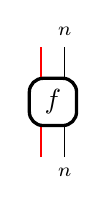
\begin{tikzpicture}[baseline=-.1cm, rotate=90]
	\draw[thick, red] (-.7,.15) -- (.7,.15);
	\draw (-.7,-.15) -- (.7,-.15);
	\roundNbox{unshaded}{(0,0)}{.3}{0}{0}{$f$}
	\node at (-.9,-.15) {\scriptsize{$n$}};
	\node at (.9,-.15) {\scriptsize{$n$}};
\end{tikzpicture}
\mapsto
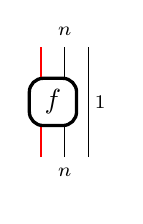
\begin{tikzpicture}[baseline=-.2cm, rotate=90]
	\draw[thick, red] (-.7,.15) -- (.7,.15);
	\draw (-.7,-.15) -- (.7,-.15);
	\draw (-.7,-.45) -- (.7,-.45);
	\roundNbox{unshaded}{(0,0)}{.3}{0}{0}{$f$}
	\node at (-.9,-.15) {\scriptsize{$n$}};
	\node at (.9,-.15) {\scriptsize{$n$}};
	\node at (0,-.6) {\scriptsize{$1$}};
\end{tikzpicture}
\end{equation}
and a trace preserving conditional expectation $E_n:A_n\rightarrow A_{n-1}$, 
\begin{equation}\label{eq:ConditionalExpectationAn}
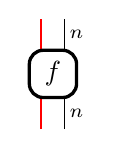
\begin{tikzpicture}[baseline=-.1cm]
	\draw[thick, red] (-.15,-.7) -- (-.15,.7);
	\draw (.15,-.7) -- (.15,.7);
	\roundNbox{unshaded}{(0,0)}{.3}{0}{0}{$f$}
	\node at (.3,.5) {\scriptsize{$n$}};
	\node at (.3,-.5) {\scriptsize{$n$}};
\end{tikzpicture}
\mapsto\,
\frac{1}{d}
\cdot
\left(\,\,
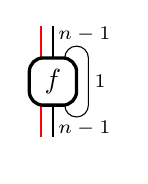
\begin{tikzpicture}[baseline=-.1cm]
	\draw[thick, red] (-.15,-.7) -- (-.15,.7);
	\draw (0,-.7) -- (0,.7);
	\draw (.15,.3) arc (180:0:.15cm) -- (.45,-.3) arc (0:-180:.15cm);
	\roundNbox{unshaded}{(0,0)}{.3}{0}{0}{$f$}
	\node at (.4,.6) {\scriptsize{$n-1$}};
	\node at (.4,-.6) {\scriptsize{$n-1$}};
	\node at (.6,0) {\scriptsize{$1$}};
\end{tikzpicture}
\right)
\end{equation}
left inverse to the inclusion.

Here, $d:=\dim_{\cC}(x)=\dim_{\cC}(\overline{x})$ the value of a closed loop appearing in the diagram. % There must be a better word for this. Maybe we should also remark why these are equal? In response: Emily peter's uses the term closed circles (on page 7 of her thesis), if that's the woridng you mean, and the equality follows from sphericality, maybe we should this should probably be in the preliminary discussion of the paragroup and the constructed multifusion category
Given the previously defined inclusion and that multiplication is given by vertical stacking of diagrams, it's clear that $E_n$ is $A_{n-1}$ bilinear. Similarly, we have that $tr_n=tr_{n-1} \circ E_n$.

Finally, the Jones projections for each inclusion $A_{n}\subset A_{n+1}$ are given by
\begin{equation}\label{eq:JonesProjections}
e_n=
\frac1d\cdot
\left(\,\,
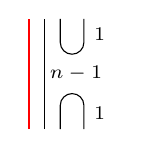
\begin{tikzpicture}[baseline=-.1cm]
	\draw[thick, red] (-.3,-.7) -- (-.3,.7);
	\draw (-.1,-.7) -- (-.1,.7);
	\draw (.1,-.7) -- (.1,-.4) arc (180:0:.15cm) -- (.4,-.7);
	\draw (.1,.7) -- (.1,.4) arc (-180:0:.15cm) -- (.4,.7);
%	\node at (-.1,-1) {\scriptsize{$n-1$}};
	\node at (.3,0) {\scriptsize{$n-1$}};
	\node at (.6,.5) {\scriptsize{$1$}};
	\node at (.6,-.5) {\scriptsize{$1$}};
\end{tikzpicture}
\right)
\in
A_{n+1}.
\end{equation}
where the $n-1$ indicates $n-1$ vertical strands with appropriate shading to the right of the red strand. The Temperley-Lieb- % strange editor enforced wordwrap from here. lint?
Jones relations follow immediately from the definition and the fact that closed loops count for a factor of $d$. Similarly, 
for any $x\in A_n$ we have $e_nxe_n=E_n(x)e_n$. Clearly, $E_{n+1}(e_n)=d^{-2}id_{m \otimes \xalt}$. Finally, the pull 
down condition % probably we should define the condition somewhere in the prelims, and then this becomes ``(some number)''; if not, then we should explicitly give the condition here, whatever it is. 
holds, as for each $x\in A_{n+1}$, we have that $d^2 E_{n+1}(xe_n)e_n=xe_n$. Equivalently, $A_{n} e_n A_n$ is a 
two-sided ideal in $A_{n+1}$. Thus, the tower algebras given by the $A_n$ is indeed a Markov sequence.
 
\begin{prop}
The Markov sequence of von Neumann Algebras $(A_n, tr_n)_{n\geq 0}$ is finite depth.
\end{prop}

\begin{proof}
	Every object of $\cM$ is a subobject of $m\otimes \xalt$ for some $n$. Let $Y^l_1,\ldots Y^l_{r_il}$, be a collection of non-isomorphic simple objects spanning $\cC_{2l}$, for $l\in\{0,1\}$. Then 

% warning: a lot of indices are undefined and text is missing in this block. 
	\[\End_{\cC}(m\otimes\xalt)\cong \bigoplus\limits_{j}\End_{\cC}(n_j Y^l_j) \cong \bigoplus\limits_{j}M_{n_j}(\bbC)\]
	At each level of the Bratteli diagram corresponding to $A_{n-1}\subseteq A_n$, 
	there are at most $\max\{r_1,r_0\}$ vertices, so the principal graph must be finite. 
\end{proof}

\begin{thm}
The principal graph obtained from the Markov sequence $(A_n, tr_n)_{n\geq 0}$ is independent of the choice of $m$, and is in fact isomorphic to the fusion graph for $\cM$.
\end{thm}

\begin{proof}
We will proceed by noting that because $x$ generates $\cC$ and $\cM$ is cyclic that we can assume there is some simple from every isomorphism class in $\cM$ appearing as a direct summand of $m\otimes \xalt $. Then our result from the fact that subsequent in inclusions $A_k\subseteq A_{k+1}$ are given by tensoring $id_x$ and $id_{\overline{x}}$ so they are determined entirely by the fusion rules.

First, recall that for a finite depth Markov sequence, the principal graph is canonically isomorphic to the Bratteli for the inclusion $A_n\subset A_{n+1}$ for $n$ large enough that this inclusion is standard, by \ref{BratteliPrincipal}. So, it suffices to show this Bratteli diagram is isomorphic to the fusion graph for $\cM$. 

Let $Y^l_1,\ldots Y^l_{r_l}$, for $l=0$ or $1$ be a collection of non-isomorphic simple objects in $\cC_{2l}$ such that every object in $\cC_{2l}$ is isomorphic to a direct sum of these elements, as in the previous proof. 
	We will work with the index $l$ mod 2 so that we may write $Y^{l+1}_j$ for brevity of notation. 
	Let the non-negative integers $p^{l}_{i,j}$ be defined by the following equation:

$$Y^l_j\otimes \act=\bigoplus\limits_{i=1}^{r_{l+1}}p_{i,j}^lY^{l+1}_i$$
where $\act$ is $x$ if $n$ is even and $\overline{x}$ if $n$ is odd. 
These coefficients are exactly the coefficients for the adjacency matrix of the fusion graph for $\act$.

Recall that:
$$A_n=\End_{\cC}(m\otimes\xalt)\cong \End_{\cC}(\bigoplus\limits_{j=1}^{r_l}n_j Y^l_j)$$
if we have that 
$$m \otimes \xalt \cong \bigoplus\limits_{j=1}^{r_l}n_jY^l_j$$
Note that we may take $n$ such that all $n_j$ are strictly positive, as there is some $n$ such that $Y^{l}_1\oplus\cdots \oplus Y^{l}_{r_l}$ is isomorphic to a direct summand of $m\otimes \xalt$ (in fact the first $n$ where this happens is exactly when the Markov sequence achieves depth). 
%But now, we know that:
%$$A_{n+1}=\End_{\cC}(m\otimes\xalt\otimes \act)\cong \End_{\cC}(\bigoplus\limits_{j=1}^{r_l}\bigoplus\limits_{i=1}^{r_{l+1}}(p_{i,j}^ln_jY^{l+1}_i))$$

The inclusion of $A_n \hookrightarrow A_{n+1}$ is given by $\phi \mapsto \phi \otimes \id_{\act}$. Each $\phi \in A_n$ is uniquely defined as a direct sum 
$$\bigoplus\limits_{j=1}^{r_l}\phi_j$$
where each $\phi_j \in \End_{\cC}(n_jY^{l}_j)$. Then, distributing tensor products over the sum, we may write $\phi$ as 
$$\bigoplus_{j=1}^{r_l}(\phi_j \otimes \id_{\act})$$
But then:
$$\phi_j \otimes \id_{\act}\in \End_{\cC}(n_jY^{l}_j\otimes \act)\cong \End_{\cC}(\bigoplus\limits_{i=1}^{r_{l+1}}p_{i,j}^ln_jY^{l+1}_i)$$
Since all $n_j\neq 0$ and the inclusion is unital, it's clear that $p_{i,j}^{l}$ gives the coefficients for the Bratteli diagram.
\end{proof}



\section{The Embedding Theorem}

\begin{claim*}
A finite depth subfactor planar algebra can be embedded into the bipartite graph planar algebra of the fusion graph obtained by right-acting the subfactor planar algebra on a cyclic module.
\end{claim*}
As was described in \cite{penneys}, one can define a canonical shaded planar *-algebra structure on the tower of relative commutants of the base of a strongly Markov tower of algebras. This planar algebra is isomorphic to the bipartite graph planar algebra of the Bratteli diagram of the first inclusion in the tower, by theorem 3.28 of \cite{penneys}. We have shown that the Markov sequence $(A_n,\tr_n)$ defined in the previous section is finite depth. Let $r$ be the minimal integer such that the inclusion $A_{2r} \subset A_{2r+1} \subset A_{2r+2}$ is standard, and let $B_n=A_{2r+n}$. Then the canonical planar *-algebra $P_\bullet$ associated to $B_0\subseteq (B_1,tr_1)$ is isomorphic to the bipartite graph planar algebra of the principle graph of the tower $\left(A_{n}\right)$; indeed, by \ref{BratteliPrincipal}, the principle graph of $(A_{n},tr_n)$ is isomorphic to the Bratteli diagram of $B_0\subseteq B_1$.
If we denote the canonical *-planar algebra associated to $B_0\subseteq(B_1,tr_1)$ by $P_{\bullet}$, then by construction, we have the following:
\begin{align*}
	P_{n,+} &=  A'_{2r}\cap A_{2r+n} \\
	P_{n,-}  &= A'_{2r+1}\cap A_{2r+n+1} 
\end{align*}

Consider the map $\Phi$, which places $2r$ strings to the left of elements in $Q_{n,+}$  and $2r+1$ strings to the left of elements in $Q_{n,-}$:
\[ 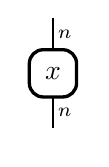
\begin{tikzpicture}[baseline]
	\draw (0,-.7) -- (0,.7);
	\roundNbox{unshaded}{(0,0)}{.3}{0}{0}{$x$}
	\node at (0.15,.5) {\scriptsize{$n$}};
	\node at (0.15,-.5) {\scriptsize{$n$}};
\end{tikzpicture}
\begin{tikzpicture}[baseline]
	\clip (0.5,0.9) -- (-0.5,0.9) -- (-0.5,-0.9) -- (0.5,-0.9);
	\draw [|->,thick] (-0.3,0)--(0.3,0);
	\node at (0,0.25) {$\Phi$};
\end{tikzpicture}
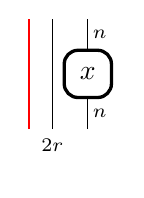
\begin{tikzpicture}[baseline]
	\draw[thick,red] (-0.3,-.7) -- (-0.3,0.7);
	\draw (0.45,-.7) -- (0.45,.7);
	\draw (0,-.7) -- (0,.7);
	\roundNbox{unshaded}{(0.45,0)}{.3}{0}{0}{$x$}
	\node at (0.6,.5) {\scriptsize{$n$}};
	\node at (0.6,-.5) {\scriptsize{$n$}};
	\node at (0,-0.9){\scriptsize{$2r$}};
\end{tikzpicture} \]
This map sends $Q_{n , +}$ to $P_{n,+}$ and $Q_{n , -}$ to $P_{n,-}$. In order to check that $\Phi(Q_{\bullet})$ is a sub $\ast$-planar algebra, we use Lemma 2.48 in the paper of Penneys and Jones. % cite
We shall state it here for the reader's convenience 
\begin{lem}[Preservation under action of tangles]
Suppose that $P_\bullet$ is a planar $\ast$-algebra with modulus $d \neq 0$ and $Q_{n,\pm} \subset P_{n,\pm}$ are $\ast$-subalgebras which are preserved by the action of the following tangles:

\begin{enumerate}[(1)]
\item Multiplication by tangles of the form $E_n = 
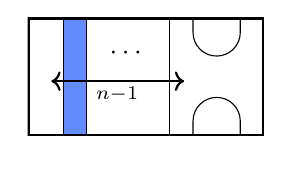
\begin{tikzpicture}[rectangular]
	\clip (2,1) --(-2,1) -- (-2,-1) -- (2,-1);
	\filldraw[shaded] (-1.4,1)--(-1.4,-1)--(-1,-1)--(-1,1);
	\draw (.4,1)--(.4,-1);
	\draw (0.8,1)--(.8,0.75) arc (-180:0:.4cm)--(1.6,1);
	\draw  (0.8,-1)--(.8,-0.75) arc (180:0:.4cm)--(1.6,-1);
	\draw [ultra thick] (2,1) --(-2,1) -- (-2,-1) -- (2,-1)--(2,1);	
	\draw[<->, thick] (-1.6,-.075) -- (0.65,-.075);
	\node at (-.475,-.3) {$_{n-1}$};
	\node at (-.3,.4) {$\cdots$};
\end{tikzpicture}
\in P_{n,+}
$
\item 
\begin{enumerate}[(i)]
\item (Right Capping) $\alpha_n = 
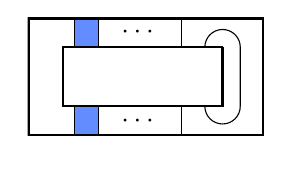
\begin{tikzpicture}[rectangular]
	\clip (2,1) --(-2,1) -- (-2,-1) -- (2,-1);
	\filldraw[shaded] (-1.2,1.5)--(-1.2,-1.5)--(-.8,-1.5)--(-.8,1.5);
	\draw (.6,1.5)--(.6,-1.5);
	\draw (1,.5) arc (180:0:.3cm) -- (1.6,-.5);
	\draw (1,-.5) arc (-180:0:.3cm);
	\draw [ultra thick] (2,1) --(-2,1) -- (-2,-1) -- (2,-1)--(2,1);
	\filldraw[thick, unshaded] (1.3,.5) --(1.3,-.5) -- (-1.4,-.5) -- (-1.4,.5)--(1.3,.5);
	\node at (-.1,.75) {$\cdots$};
	\node at (-.1,-.75) {$\cdots$};
	\node at (-.05,0) {};
\end{tikzpicture}
: P_{n,+} \to P_{n-1,+}
$
\item (Inclusion) $\beta_n = 
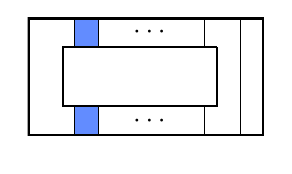
\begin{tikzpicture}[rectangular]
	\clip (2,1) --(-2,1) -- (-2,-1) -- (2,-1);
	\filldraw[shaded] (-1.2,1.5)--(-1.2,-1.5)--(-.8,-1.5)--(-.8,1.5);
	\draw (1.6,1.5)--(1.6,-1.5);
	\draw (1,1.5) --(1,-1.5);
	\draw [ultra thick] (2,1) --(-2,1) -- (-2,-1) -- (2,-1)--(2,1);
	\filldraw[thick, unshaded] (1.2,.5) --(1.2,-.5) -- (-1.4,-.5) -- (-1.4,.5)--(1.2,.5);
	\node at (0.1,.75) {$\cdots$};
	\node at (0.1,-.75) {$\cdots$};
	\node at (-0.1,0) {};
\end{tikzpicture}
: P_{n,+} \to P_{n+1,+}
$
\item (Left Capping) $\gamma^{+}_n =
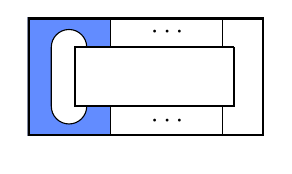
\begin{tikzpicture}[rectangular]
	\clip (2,1) --(2,-1) -- (-2,-1) -- (-2,1);
	\filldraw[shaded] (-2.5,1.5)--(-2.5,-1.5)--(-.6,-1.5)--(-.6,1.5);
	\draw (1.3,1.5)--(1.3,-1.5);
	\filldraw[unshaded] (-1,.5) arc (0:180:.3cm) -- (-1.6,-.5) arc (-180:0:.3cm) -- (-1,.5);
	\draw [ultra thick] (2,1) --(-2,1) -- (-2,-1) -- (2,-1)--(2,1);
	\filldraw[thick, unshaded] (1.5,.5) --(1.5,-.5) -- (-1.2,-.5) -- (-1.2,.5)--(1.5,.5);
	\node at (.4,.75) {$\cdots$};
	\node at (.4,-.75) {$\cdots$};
	\node at (.15,0) {};
\end{tikzpicture}
: P_{n,+} \to P_{n-1,-}
$ 
\end{enumerate}
\item (Left inclusion) $i^{-}_n =
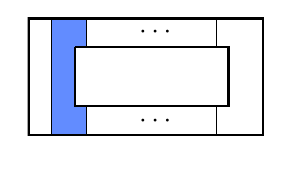
\begin{tikzpicture}[rectangular]
	\clip (2,1) --(-2,1) -- (-2,-1) -- (2,-1);
	\filldraw[shaded] (-1.6,1.5)--(-1.6,-1.5)--(-1,-1.5)--(-1,1.5);
	\draw (1.2,1.5)--(1.2,-1.5);
	\draw [ultra thick] (2,1) --(-2,1) -- (-2,-1) -- (2,-1)--(2,1);
	\filldraw[thick, unshaded] (-1.2,.5) --(-1.2,-.5) -- (1.4,-.5) -- (1.4,.5)--(-1.2,.5);
	\node at (0.2,.75) {$\cdots$};
	\node at (0.2,-.75) {$\cdots$};
	\node at (0.1,0) {};
\end{tikzpicture}
: P_{n,-} \to P_{n+1,+}
$ 
\end{enumerate}
Then the $Q_{n,\pm}$ are preserved under every tangle and thus form a planar $\ast$-subalgebra $Q_\bullet \subset P_\bullet$
\end{lem}
We denote traces in $Q_{\bullet}$ by $\overline{\tr}$ and traces in $P_{\bullet}$ by $\tr$. We denote the Jones projections in $Q_{\bullet}$ by $E_{j}$ and the Jones projections in  $P_{\bullet}$ by $F_{j}$.


\begin{thm}
The image of the map $\Phi:Q_{\bullet} \to P_{\bullet}$ is a $\ast$-planar subalgebra of $P_{\bullet}$.
\end{thm} 

\begin{proof}
Observe that for all $x,y \in Q_{\bullet}$, we have that 
\begin{align*}
	\Phi(x^{*}) &= \Phi(x)^{\ast} \\
	\Phi(xy) &= \Phi(x)\Phi(y) \\
	\overline{\tr}_{n}(x) &= \frac{1}{\dim_\cC(x)^{2r}}\cdot\tr_{n}(\Phi(x)) 
\end{align*}

	To prove the injectivity of $\Phi$, we can use the faithfullness of the traces and the third equation displayed above. % confusing. Number (or name) your equations for clarity in this situation. 
	In section \todo{Cover how the relative commutant algebra looks} we see that in the relative commutant planar algebra, the tangles described in Lemma 2.48 are associated to well known functions! Thus we can check that $\Phi(Q_\bullet)$ is preserved under the specified tangles by using both algebraic and pictorial relations. We now proceed to check the requirements of Lemma 2.48  
\begin{enumerate}[(1)]
\item By the construction of $P_{\bullet}$, we have that $\Phi(E_j)=F_j$. Thus, $\Phi(Q_{n,\pm})$ is closed under multiplication by Jones projections. 
\item \begin{enumerate}[(i)]
\item We have that $\Phi(E_n(x)) = E_{2r+n}(\Phi(x))$. This follows from the graphical calculi in both the domain and range. Note that $E_{2r+n | Q'_{2r}\cap Q_{2r+n}} = E_{P_{n,+}}$ because they are both faithful trace preserving conditional expectations on $P_{n,+}$.
\item We have that $\Phi(\beta_n(x)) = \beta_{2r+n}(\Phi(x))$ due to graphical calculi in the domain and range. Also note that the inclusion from $P_{n,+} \to P_{n+1,+}$ is just the restriction of the incusion from $Q_{2r+n,+} \to Q_{2r+n+1,+}$. 
\item In the section \todo{Section with Rel com algebra} we showed that the left capping tangle $\gamma_n$ in the relative commutant planar algebra was algebraically described as:
\[
 \gamma^{+}_n(x) = \frac{1}{d^2}\sum_{b \in B}bxb^\ast
\]
where $B$ is a Pimnser Popa basis of $B_1$ over $B_0$. We will now check that $\gamma^{+}_n$ preserves $\Phi(Q_{\bullet})$. For any $x \in Q_{n,+}$, we have 

\centerline{
  \begin{minipage}{\linewidth}
			\[
				d^2\gamma^+_n(\Phi(x))
				=
\sum_{b\in B}
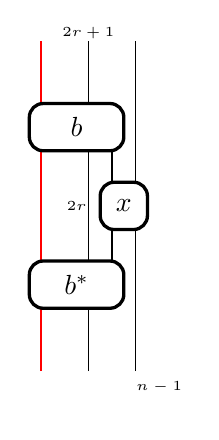
\begin{tikzpicture}[baseline]
	\draw[thick,red] (-0.6,-2.1) -- (-0.6,2.1);
	\draw (0.6,-2.1) -- (0.6,2.1);
	\draw (0.3,-.7) -- (0.3,.7);
	\draw (0,-2.1) -- (0,2.1);
	\roundNbox{unshaded}{(0.45,0)}{.3}{0}{0}{$x$}
	\roundNbox{unshaded}{(0.15,1)}{.3}{0.6}{0}{$b$}
	\roundNbox{unshaded}{(0.15,-1)}{.3}{0.6}{0}{$b^\ast$}
	\node at (0.9,-2.3) {\tiny{$n-1$}};
	\node at (0,2.2) {\tiny{$2r+1$}};
	\node at (-.15,0) {\tiny{$2r$}};
\end{tikzpicture} 
=
\sum_{b\in B}
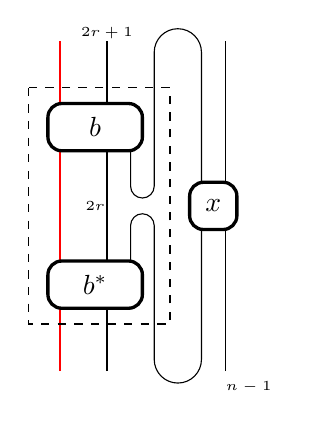
\begin{tikzpicture}[baseline]
	\draw[thick,red] (-0.6,-2.1) -- (-0.6,2.1);
	\draw (0.3,.7)--(0.3,0.25) arc (-180:0:.15cm)-- (0.6,1.95) arc(180:0:.3cm) -- (1.2,.15);
	\draw (0.3,-.7)--(0.3,-0.25) arc (180:0:.15cm)-- (0.6,-1.95) arc(-180:0:.3cm) -- (1.2,-.15);
	\draw (0,-2.1) -- (0,2.1);
	\draw (1.5,-2.1) -- (1.5,2.1);
	\draw[dashed] (-1,1.5) --  (-1,-1.5) --  (0.8,-1.5) --  (0.8,1.5) -- (-1,1.5);
	\roundNbox{unshaded}{(1.35,0)}{.3}{0}{0}{$x$}
	\roundNbox{unshaded}{(0.15,1)}{.3}{0.6}{0}{$b$}
	\roundNbox{unshaded}{(0.15,-1)}{.3}{0.6}{0}{$b^\ast$}
	\node at (1.8,-2.3) {\tiny{$n-1$}};
	\node at (0,2.2) {\tiny{$2r+1$}};
	\node at (-.15,0) {\tiny{$2r$}};
\end{tikzpicture} 
=
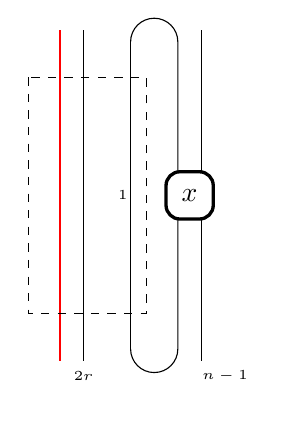
\begin{tikzpicture}[baseline]
	\draw[thick,red] (-0.3,-2.1) -- (-0.3,2.1);
	\draw (0.6,1.95) arc(180:0:.3cm) -- (1.2,.15);
	\draw (0.6,-1.95) arc(-180:0:.3cm) -- (1.2,-.15);
	\draw (0.6,1.95) -- (0.6,-1.95);
	\draw (0,-2.1) -- (0,2.1);
	\draw (1.5,-2.1) -- (1.5,2.1);
	\draw[dashed] (-0.7,1.5) --  (-0.7,-1.5) --  (0.8,-1.5) --  (0.8,1.5) -- (-0.7,1.5);
	\roundNbox{unshaded}{(1.35,0)}{.3}{0}{0}{$x$}
	\node at (1.8,-2.3) {\tiny{$n-1$}};
	\node at (0,-2.3) {\tiny{$2r$}};
	\node at (0.5,0) {\tiny{$1$}};
\end{tikzpicture} 
=
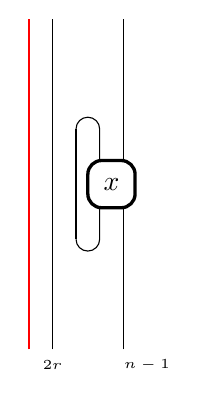
\begin{tikzpicture}[baseline]
	\draw[thick,red] (-0.3,-2.1) -- (-0.3,2.1);
	\draw (0.3,0.7) arc(180:0:.15cm) -- (0.6,.15);
	\draw (0.3,-0.7) arc(-180:0:.15cm) -- (0.6,-.15);
	\draw (0.3,0.7) -- (0.3,-0.7);
	\draw (0,-2.1) -- (0,2.1);
	\draw (0.9,-2.1) -- (0.9,2.1);
	\roundNbox{unshaded}{(0.75,0)}{.3}{0}{0}{$x$}
	\node at (1.2,-2.3) {\tiny{$n-1$}};
	\node at (0,-2.3) {\tiny{$2r$}};
\end{tikzpicture}
	\]
  \end{minipage}
}
Clearly, the last diagram depicts an element of  $\Phi(Q_{\bullet})$.
\end{enumerate}
\item The negative inclusion $i^{-}_{n} : P_{n,-} \to P_{n+1,+}$ is just the identity on the relative commutant planar algebra. Let $\overline{i^{-}_{n}}$ be the negative inclusion in $Q_{n,\pm}$. Graphically, this is equivalent to adding a string on the left. Thus, for $x$ in $Q_{n,-}$ we have that:
\[
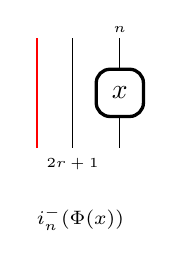
\begin{tikzpicture}[baseline]
	\draw[red, thick] (-0.9,-0.7) -- (-0.9,0.7);
	\draw (-0.45,-0.7) -- (-0.45,0.7);
	\draw (0.15,-0.7) -- (0.15,0.7);
	\roundNbox{unshaded}{(0.15,0)}{.3}{0}{0}{$x$};
	\node at (0.15,0.8){\tiny{$n$}};
	\node at (-0.45, -0.9){\tiny{$2r+1$}};
	\node at (-0.35,-1.6){\scriptsize{$ i^{-}_{n}(\Phi(x))$}};
\end{tikzpicture}
\quad
=
\quad
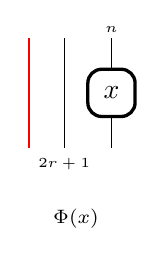
\begin{tikzpicture}[baseline]
	\draw[red, thick] (-0.9,-0.7) -- (-0.9,0.7);
	\draw (-0.45,-0.7) -- (-0.45,0.7);
	\draw (0.15,-0.7) -- (0.15,0.7);
	\roundNbox{unshaded}{(0.15,0)}{.3}{0}{0}{$x$};
	\node at (0.15,0.8){\tiny{$n$}};
	\node at (-0.45, -0.9){\tiny{$2r+1$}};
	\node at (-0.30,-1.6){\scriptsize{$\Phi(x)$}};
\end{tikzpicture}
\quad
=
\quad
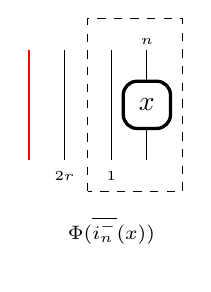
\begin{tikzpicture}[baseline]
	\draw[red, thick] (-0.9,-0.7) -- (-0.9,0.7);
	\draw (-0.45,-0.7) -- (-0.45,0.7);
	\draw (0.6,-0.7) -- (0.6,0.7);
	\draw (0.15,-0.7) -- (0.15,0.7);
	\roundNbox{unshaded}{(.6,0)}{0.3}{0}{0}{$x$};
	\draw[dashed] (-0.15,-1.1) -- (-0.15,1.1) -- (1.05,1.1) --  (1.05,-1.1) -- (-0.15,-1.1);
	\node at (0.6,0.8){\tiny{$n$}};
	\node at (-0.45, -0.9){\tiny{$2r$}};
	\node at (0.15,-0.9){\tiny{1}};
	\node at (0.15,-1.6){\scriptsize{$\Phi(\overline{i^{-}_{n}}(x))$}};
\end{tikzpicture}\]
\end{enumerate}
\end{proof}

We have checked that $\Phi(Q_{\bullet}) \subset P_{\bullet}$ is a $\ast$-planar algebra inclusion. Let $G_\bullet$ be the bipartite graph planar algebra on the principle graph of $(A_n)$. Then by Theorem 3.33 in the paper of Penneys and Jones, % cite
we have that $P_\bullet$ is $\ast$-planar algebra isomorphic to $G_\bullet$. Thus, we have successfully embedded $Q_\bullet$ into $G_\bullet$.

\begin{cor}[The Embedding Theorem]
	A subfactor planar algebra $Q_\bullet$ can be embedded into the bipartite graph planar algebra of the principle graph of a cyclic $Q_\bullet$-module.
\end{cor}



\bibliographystyle{plain}
\bibliography{shredthegnar}
\end{document}
